\documentclass[a4paper, 12pt, twoside]{article}


%------------------------------------------------------------------------
%
% Author                :   Lasercata
% Last modification     :   2022.05.23
%
%------------------------------------------------------------------------


%------ini
\usepackage[utf8]{inputenc}
\usepackage[T1]{fontenc}
\usepackage[french]{babel}
%\usepackage[english]{babel}


%------geometry
\usepackage[textheight=700pt, textwidth=500pt]{geometry}


%------color
\usepackage{xcolor}
\definecolor{ff4500}{HTML}{ff4500}
\definecolor{00f}{HTML}{0000ff}
\definecolor{0ff}{HTML}{00ffff}
\definecolor{656565}{HTML}{656565}

\renewcommand{\emph}{\textcolor{ff4500}}
\renewcommand{\em}{\color{ff4500}}

\newcommand{\strong}[1]{\textcolor{ff4500}{\bf #1}}
\newcommand{\st}{\color{ff4500}\bf}


%------Code highlighting
\usepackage{listings}

\definecolor{cbg}{HTML}{272822}
\definecolor{cfg}{HTML}{ececec}
\definecolor{ccomment}{HTML}{686c58}
\definecolor{ckw}{HTML}{f92672}
\definecolor{cstring}{HTML}{e6db72}
\definecolor{cstringlight}{HTML}{98980f}
\definecolor{lightwhite}{HTML}{fafafa}

\lstdefinestyle{DarkCodeStyle}{
    backgroundcolor=\color{cbg},
    commentstyle=\itshape\color{ccomment},
    keywordstyle=\color{ckw},
    numberstyle=\tiny\color{cbg},
    stringstyle=\color{cstring},
    basicstyle=\ttfamily\footnotesize\color{cfg},
    breakatwhitespace=false,
    breaklines=true,
    captionpos=b,
    keepspaces=true,
    numbers=left,
    numbersep=5pt,
    showspaces=false,
    showstringspaces=false,
    showtabs=false,
    tabsize=4,
    xleftmargin=\leftskip
}

\lstdefinestyle{LightCodeStyle}{
    backgroundcolor=\color{lightwhite},
    commentstyle=\itshape\color{ccomment},
    keywordstyle=\color{ckw},
    numberstyle=\tiny\color{cbg},
    stringstyle=\color{cstringlight},
    basicstyle=\ttfamily\footnotesize\color{cbg},
    breakatwhitespace=false,
    breaklines=true,
    captionpos=b,
    keepspaces=true,
    numbers=left,
    numbersep=10pt,
    showspaces=false,
    showstringspaces=false,
    showtabs=false,
    tabsize=4,
    frame=L,
    xleftmargin=\leftskip
}

%\lstset{style=DarkCodeStyle}
\lstset{style=LightCodeStyle}

%Usage : \begin{lstlisting}[language=Caml] ... \end{lstlisting}



%-make the table of content clickable
\usepackage{hyperref}
\hypersetup{
    colorlinks,
    citecolor=black,
    filecolor=black,
    linkcolor=black,
    urlcolor=black
}


%------pictures
\usepackage{graphicx}
%\usepackage{wrapfig}


%------tabular
%\usepackage{color}
%\usepackage{colortbl}
%\usepackage{multirow}


%------Physics
%---Packages
%\usepackage[version=4]{mhchem} %$\ce{NO4^2-}$

%---Commands
\newcommand{\link}[2]{\mathrm{#1} \! - \! \mathrm{#2}}
\newcommand{\pt}[1]{\cdot 10^{#1}} % Power of ten
\newcommand{\dt}[2][t]{\dfrac{d#2}{d#1}} % Derivative


%------math
%---Packages
%\usepackage{textcomp}
%\usepackage{amsmath}
\usepackage{amssymb}
\usepackage{mathtools} % For abs
\usepackage{stmaryrd} %for \llbracket and \rrbracket
\usepackage{mathrsfs} %for \mathscr{x} (different from \mathcal{x})

%---Commands
%-Sets
\newcommand{\N}{\mathbb{N}} %set N
\newcommand{\R}{\mathbb{R}} %set R
\newcommand{\C}{\mathbb{C}} %set C
\newcommand{\U}{\mathbb{U}} %set U
\newcommand{\set}[2]{\left[ #1\ ;\ #2 \right]}
\newcommand{\nset}[2]{\left\llbracket #1\ ;\ #2 \right\rrbracket}

%-Exponantial / complexs
\newcommand{\e}[1]{\mathrm{e}^{#1}}
\newcommand{\ex}{\e{x}}
\newcommand{\eit}{\e{i\theta}}
\newcommand{\cj}[1]{\overline{#1}} %overline for the conjugate.
\newcommand{\cjz}{\cj{z}} %conjugate of z

%-Vectors
\newcommand{\vect}{\overrightarrow}
\newcommand{\veco}[3]{\displaystyle \vect{#1}\binom{#2}{#3}} %vector + coord

%-Limits
\newcommand{\lm}[2][{}]{\lim\limits_{\substack{#2 \\ #1}}} %$\lm{x \to a} f$ or $\lm[x < a]{x \to a} f$
\newcommand{\Lm}[3][{}]{\lm[#1]{#2} \left( #3 \right)} %$\Lm{x \to a}{f}$ or $\Lm[x < a]{x \to a}{f}$

%-Integral
\newcommand{\dint}[4][x]{\displaystyle \int_{#2}^{#3} #4 \mathrm{d} #1} %$\dint{a}{b}{f(x)}$ or $\dint[t]{a}{b}{f(t)}$

%-Others
\newcommand{\trig}[2]{#1 \left( #2 \right)} %$\trig{\sin}{\dfrac a b}$
\newcommand{\para}{\ /\!/\ } %//
\newcommand{\ssi}{\ \Leftrightarrow \ }
\newcommand{\abs}[1]{\left\lvert #1 \right\rvert} % abs{x} -> |x|
\newcommand{\eqsys}[2]{\begin{cases} #1 \\ #2 \end{cases}}

\newcommand{\med}[2]{\mathrm{med} \left[ #1\ ;\ #2 \right]}  %$\med{A}{B} -> med[A ; B]$
\newcommand{\Circ}[2]{\mathscr{C}_{#1, #2}}

\newcommand{\lr}[1]{\left( #1 \right)}
\newcommand{\lrb}[1]{\left[ #1 \right]}

\newcommand{\lrangle}[1]{\left\langle #1 \right\rangle}


%------commands
%---to quote french text
\newcommand{\simplecit}[1]{\guillemotleft$\;$#1$\;$\guillemotright}
\newcommand{\cit}[1]{\simplecit{\textcolor{656565}{#1}}}
\newcommand{\quo}[1]{\cit{\it #1}}

%---to indent
\newcommand{\ind}[1][20pt]{\advance\leftskip + #1}
\newcommand{\deind}[1][20pt]{\advance\leftskip - #1}

%---to indent a text
\newcommand{\indented}[2][20pt]{\par \ind[#1] #2 \par \deind[#1]}
\newenvironment{indentedenv}[1][20pt]{\par \ind[#1]}{\par \deind}
\newenvironment{indt}[2][20pt]{#2 \begin{indentedenv}[#1]}{\end{indentedenv}} %Titled indented env

%---title
\newcommand{\thetitle}[2]{\begin{center}\textbf{{\LARGE \underline{\emph{#1} :}} {\Large #2}}\end{center}}

%---parts
%-I
\newcommand{\mainpart}[2][$\!\!$]{\underline{\large \textbf{\emph{\textit{#1} #2}}}}
\newcommand{\bmainpart}[2][$\!\!$]{\underline{\large \textbf{\textit{#1} #2}}}
%-A
\newcommand{\subpart}[2][$\!\!$]{.\underline{\bf \textit{#1} #2}}
%-1
\newcommand{\subsubpart}[2][$\!\!$]{.\underline{\textsl{#1} #2}}
%-a
\newcommand{\subsubsubpart}[2][$\!\!$]{.\underline{\it #1 #2}}

%math part
\newcommand{\secpart}[1]{.\underline{\it #1 :}}

\newenvironment{mathdef}[2][20pt]{
    \secpart{#2} \begin{indentedenv}[#1]}
    {\end{indentedenv}}


%------page style
\usepackage{fancyhdr}
\usepackage{lastpage}

\setlength{\headheight}{18pt}
\setlength{\footskip}{50pt}

\pagestyle{fancy}
\fancyhf{}
\fancyhead[LE, RO]{\textit{\today}}
\fancyhead[RE, LO]{\large{\textsl{\emph{\texttt{\jobname}}}}}

\fancyfoot[RO, LE]{\textit{\texttt{Page \thepage /\pageref{LastPage}}}}
\fancyfoot[LO, RE]{\includegraphics[scale=0.12]{/home/lasercata/Pictures/1.images_profil/logo/mieux/lasercata_logo_fly_fond_blanc.png}}


%------init lengths
\setlength{\parindent}{0pt} %no \noindent needed !!!
\setlength{\parskip}{3pt}


%-----------------------------------Begin Document
\begin{document}

    \thetitle{Chap 2}{Représentation et stockage de l'information}
    
    \tableofcontents
    \newpage
    
    
    \begin{indt}{\section{Mémoire d'un programme compilé :}}
        
        \begin{indt}{\subsection{Organisation de la mémoire}}
            
            \begin{indt}{\subsubsection{Distinction statique dynamique}}

                \begin{indt}{Le stockage des objets manipulés par un programme est géré de deux manières différentes selon leur nature :}
                    $-$ Statiquement : lorsque le compilateur dispose de l'information suffisante pour prévoir de la place pour ces données, elle peut être réservée à l'avance ;
                    
                    \vspace{6pt}
                    
                    $-$ Dynamiquement : lorsque la taille des objets n'est connue que lors de l'éxécution du programme, le programme doit faire une demande d'allocation pour obtenir l'espace en mémoire
                \end{indt}
                
                \vspace{6pt}
                    
                Ex : les variables globales / locales constantes ou dont la taille est fixée (ex type \texttt{int}, \texttt{char}) sont gérées statiquement.
                Les tableau dont la taille dépend de l'état du programme au moment de l'éxécution (ex : \texttt{Array.make n 0} : \texttt n est variable) sont gérés dynamiquement.
                
                \vspace{6pt}
                
                \begin{indt}{$\bullet$ Allocation statique : plusieurs zones de mémoire sont utilisées selon la nature de l'objet :}
                    $-$ Variables globales \textit{initialisées} : stockées dans le binaire donc chargé en mémoire avec le binaire dans une zone spécifique qui l'accompagne.
                    
                    \vspace{6pt}
                    
                    $-$ Les variables globales \textit{non initialisées} sont allouées, placées en mémoire au moment du chargement du binaire qui ne contient que leur déclaration.
                    
                    \vspace{6pt}
                    
                    $-$ Les variables locales et dont les paramètres des fonctions sont placées dans une zone mémoire spécifique appelée pile, utilisée dynamiquement afin de ne réserver l'espace qu'au moment de l'appel de fonction ou de l'éxécution du bloc
                \end{indt}
                
                \vspace{12pt}
                
                $\bullet$ Allocation dynamique : on utilise une zone spécifique appelée \textit{tas}
                
                Les détails spécifiques aux langages C et OCaml seront vus en 1.2.
                
                \vspace{6pt}
                
                Schéma :
                
                \begin{tabular}{c}
                    
                    \hline
                    Code binaire
                    \\
                    \hline
                    Variables globales initialisées
                    \\
                    \hline
                    variables globales non initialisées
                    \\
                    \hline
                    tas (heap)
                    \\
                    $\downarrow$
                    \\
                    \hline
                    $\uparrow$
                    \\
                    Pile (stack)
                    \\
                    \hline
                \end{tabular}
                
                \vspace{12pt}
                
                Commande : \texttt{objdump}
                Ex : \texttt{gcc -c prog.c}
                puis
                \texttt{objdump -x prog.o}
                
                %\vspace{64pt}
            \end{indt}
        
            %\vspace{6pt}
            
            \begin{indt}{\subsubsection{Portée syntaxique d'un identificateur}}
                Def : la portée syntaxique d'un identificateur est la zone de texte d'un programme dans laquelle il est possible d'y faire référence sans erreur à la compilation
                
                Ex :
                \begin{lstlisting}[language=C, xleftmargin=80pt]
int a = 1;
int f(int x) {
    int y = x + a;
    return y;
}
int g() {
    int z = 3;
    return z + f(z);
}
                \end{lstlisting}
                
                \begin{tabular}{c|c}
                    Identificateur
                    & Portée
                    \\
                    \hline
                    a & 1-9
                    \\
                    x & 2-5
                    \\
                    y & 3-5
                    \\
                    f & 2-9
                    \\
                    z & 7-9
                    \\
                    g & 6-9
                \end{tabular}
                
                Attention, la portée est associée aux identificateurs, pas aux variables.
                
                Ex :
                \begin{lstlisting}[language=C, xleftmargin=80pt]
int f() {
    int i = 3;
    return i;
}

int g() {
    int i = 5;
    return i + 1;
}
                \end{lstlisting}
                
                Portée de \texttt{i} : 2-4 et 6-8
                
                Même identificateur donc même portée pour deux variables bien distinctes.
                
                \vspace{6pt}
                
                \begin{lstlisting}[language=C, xleftmargin=80pt]
int f() {
    int i = 3;
    for (int j = 0 ; j < 3 ; j ++) {
        int i = 4;
        i = i + j;
    }
    return i;
}
                \end{lstlisting}
                
                Portée de \texttt{i} : 2-8
                
                Mais phénomène de masquage dans les lignes 4-6.
                
                \vspace{6pt}
                
                Rq : les mêmes principes s'appliquent en OCaml sauf qu'il est impossible de faire référence à une variable non initialisée.
                
                Pour ces deux langages, la portée est statique. En Python, la portée est dynamique.
            \end{indt}
            
            \vspace{6pt}
            
            \begin{indt}{\subsubsection{Durée de vie d'une variable}}
                Def : la durée de vie d'une variable correspond à la période de l'éxécution du programme depuis son allocation jusqu'a la libération de la mémoire associée.
                
                \vspace{6pt}
                
                Rq : la plupart du temps, la durée de vie d'une variable correspond à la portée de son identificateur.
                
                \vspace{6pt}
                
                En C, il est possible de définir des variables, dites statiques, dont la durée de vie dépasse la portée (H.P).
            \end{indt}
            
            \vspace{6pt}
            
            \begin{indt}{\subsubsection{Gestion de la pile}}
                La pile sert au stockage des variables locales et des paramètres des fonctions. Son remplissage évolue en fonction de l'éxécution du programme en ``empilant'' les zones crées, et en ``dépilant'' les zones libérées, à la manière de la structure de données appelée pile (cf plus tard)
                
                \vspace{6pt}
                
                Rq : on peut utiliser les registres du processeur pour stocker certaines données. On suppose ici que ce n'est pas le cas.
                
                \vspace{6pt}
                
                \begin{indt}{Lors d'un appel de fonction, on ajoute sur la pile d'éxécution un bloc de mémoire (stack frame) correspondant au bloc d'activation de la fonction, qui contient :}
                    $-$ Les paramètres de la fonction ;
                    
                    $-$ L'adresse de retour, indiquant la position à laquelle doit reprendre l'éxécution du programme après l'éxécution de la fonction ;
                    
                    $-$ Un espace pour le résultat de la fonction, qui sera transmis ;
                    
                    $-$ De l'espace pour les variables locales ;
                    
                    $-$ L'adresse du bloc précédant, permettant de dépiler le bloc d'activation après l'éxécution de la fonction.
                \end{indt}
                
                \vspace{6pt}
                
                Ex :            
                \begin{lstlisting}[language=C, xleftmargin=80pt]
int f(int a, int b) {
    int c = 3;
    c = c + b;
    c = c * a;
    return c;
}

int main() {
    int x = f(10, 12);
    return 0;
}
                \end{lstlisting}
                
                \begin{tabular}{rll}
                    f
                    &
                    \fbox{
                        \begin{tabular}{l}
                        \fbox{} retour (adresse)
                        \\
                        \fbox{150} retour (valeur)
                        \\
                        \fbox{150} c \fbox{10}$^a$ \fbox{12}$^b$
                        \\
                        \fbox{adr$_2$} bloc précédent
                        \end{tabular}
                    }
                    \\
                    \texttt{main}
                    &
                    \fbox{
                        \begin{tabular}{l}
                        \fbox{} retour (adresse)
                        \\
                        \fbox{$\bullet$} retour (valeur)
                        \\
                        \fbox{150} $x$ \fbox{adr$_1$ bloc précédant}
                        \end{tabular}
                    }
                    \\
                    &&$^{\text{adr}_1}$
                \end{tabular}
                
                \vspace{12pt}
                
                Attention, la pile est limitée : s'il y a trop d'appels de fonction imbriqués, l'empilement des blocs d'activation dépassera la capacité de la pile (Stack overflow)
                
                Ex : une fonction récursive sans cas de base (boucle infinie) ou qui fait trop d'appels récursifs.
                
                \begin{lstlisting}[language=Caml, xleftmargin=80pt]
let rec sum (n : int) : int =
    match n with
    | 0 -> 0
    | _ -> n + sum (n - 1)
                \end{lstlisting}
                
                \begin{tabular}{rl}
                    sum
                    & \fbox{
                        \begin{tabular}{l}
                        \fbox{49} n
                        \\
                        $\square$ res
                        \\
                        $\square$ retour
                        \\
                        \fbox{adr1} adr bloc
                        \end{tabular}
                    }
                    \\
                    sum
                    & \fbox{
                        \begin{tabular}{l}
                        \fbox{50} n
                        \\
                        $\square$ res
                        \\
                        $\square$ retour
                        \\
                        \fbox{adr1} adr bloc
                        \end{tabular}
                    }
                \end{tabular}
                
                \begin{lstlisting}[language=Caml, xleftmargin=80pt]
let sum (n : int) =
    let rec aux (n : int) (acc : int) =
        match n with
        | 0 -> acc
        | _ -> aux (n - 1) (acc + n) (*The calculation is in the args : the stack frame will not be kept.*)
    in aux n 0;;
                \end{lstlisting}
                
                Optimisation pour les fonctions récursives terminales en OCaml.
                Pas garantit en C.
                Pas faite en Python.
            \end{indt}
            
        \end{indt}
        
        \vspace{12pt}
        
        \begin{indt}{\subsection{Gestion de la mémoire en OCaml et en C}}
            
            \begin{indt}{\subsubsection{Gestion de la mémoire en OCaml}}
                En OCaml, la gestion de la mémoire est gérée automatiquement, les allocations dynamiques sont réalisées de manière transparente (comme toutes les déclarations). La mémoire est également libérée automatiquement grâce à un programme appelé \textit{garbage collector} (ramasse-miette / glaneur de cellules) qui détecte quand un bloc de mémoire peut être libéré et qui réorganise le tas pour le compacter.
            \end{indt}
            
            \vspace{6pt}
            
            \begin{indt}{\subsubsection{Principe de gestion de la mémoire en C}}
                Contrairement à OCaml, les allocations dynamiques en C sont gérées par le programmeur qui doit réclamer explicitement l'allocation d'un bloc mémoire sur le tas d'une taille donnée et qui doit signaler plus tard au système que la mémoire peut être libérée. Il faut impérativement libérer toute mémoire allouée.
                
                Dans le cas contraire, on parle de \textit{fuite mémoire} et le système peut devenir innutilisable faute de mémoire disponible.
                
                En C, on fait référence aux zones de mémoire par leur adresse.
            \end{indt}
            
            \vspace{6pt}
            
            \begin{indt}{\subsubsection{Pointeurs}}
                Les pointeurs sont des objets qui représentent des adresses en mémoire. \`A la manière des références en OCaml, le type des pointeurs est paramétré par le type de la valeur contenue dans le bloc mémoire qu'ils adressent / sur laquelle ils pointent.
                
                Syntaxe : \texttt{<type>*} est le type des pointeurs qui pointent sur ine valeur de type \texttt{<type>}.
                
                Déclaration : Comme pour les autres variables.
                
                Ex :
                
                \begin{lstlisting}[language=C, xleftmargin=80pt]
int *p;
double **q;\end{lstlisting}
                
                Rq : on peut placer l'étoile contre le type ou contre le nom de la variable ou même séparée des deux par des espaces.
                
                Attention : \texttt{int* p, a;} déclare un pointeur sur entier \texttt{p} et un entier \texttt{a}.
                
                \vspace{12pt}
                
                $\bullet$ Opérateur d'adressage : c'est \texttt{\&}.
                
                Rappel : \texttt{scanf} prend une adresse en argument.
                
                Ex :
                \begin{lstlisting}[language=C, xleftmargin=80pt]
int a = 2;
int* p = &a;\end{lstlisting}
                
                \vspace{12pt}
                
                $\bullet$ Opérateur de déréférencement : c'est \texttt{*}.
                
                Ex : après l'ex précédent, \texttt{*p} vaut 2.
                
                On peut voir le déréférencement de \texttt p comme une variable dont on peut modifier la valeur.
                
                Ex :
                \begin{lstlisting}[language=C, xleftmargin=80pt]
*p = 3;
printf("%d\n", a); //affiche 3\end{lstlisting}
                
                \vspace{12pt}
                
                On peut utiliser les pointeurs pour écrire des fonctions qui renvoient plusieurs résultats.
                Idée : on écrit une fonction de type \texttt{void} qui prend en paramètres des pointeurs sur les cases mémoires où l'on souhaite récupérer les résultats.
                
                Ex :
                \begin{lstlisting}[language=C, xleftmargin=80pt]
void minx_max(int x, int y, int *min, int *max) {
    if (x <= y) {
        *min = x;
        *max = y;
    }
    else {
        *min = y;
        *max = x;
    }
}

int x = 5, y = -8;
min_max(x, y, &x, &y);\end{lstlisting}
                
                Pour afficher un pointeur avec \texttt{printf}, on utilise \texttt{\%p}.
            \end{indt}
            
            \vspace{6pt}
            
            \begin{indt}{\subsubsection{Allocation dynamique en C}}
                 \begin{indt}{On dispose de deux fonctions :}
                    $-$ \emph{Allocation} : on utilise la fonction \texttt{\em malloc}, de prototype
                    \newline
                    \texttt{void* malloc(size\_t size)}.
                    
                    \texttt{void*} : pointeur sur ``rien'' (on ne connait pas le type de la valeur sur laquelle le pointeur pointe) ;
                    
                    \texttt{size\_t} : type représentant une taille.
                    
                    On utilise le transtypage pour choisir le type du pointeur.
                    
                    Ex : \texttt{char *t = (char*) malloc(n);}
                    
                    En cas d'échec de l'allocation, \texttt{malloc} renvoit un pointeur particulier, noté \texttt{NULL}
                    
                    Pour déterminerle nombre d'octets à allouer, on utilise la fonction \texttt{sizeof} qui prend en paramètre un type ou un objet et qui renvoit sa taille.
                    
                    Ex :
                    \begin{lstlisting}[language=C, xleftmargin=100pt]
int *t = (int*) malloc(n * sizeof(int));\end{lstlisting}
                    
                    \vspace{12pt}
                    
                    $-$ \emph{Libération} : on utilise la fonction \texttt{\em free}, de prototype \texttt{void free(void* ptr)}.
                    
                    \texttt{void} : c'est une instruction ;
                    
                    \texttt{void* ptr} : on peut prendre n'importe quel pointeur (par transtypage).
                    
                    Ex : \texttt{free(t);}
                \end{indt}
                
                \vspace{12pt}
                
                Attention :
                
                \begin{lstlisting}[language=C, xleftmargin=80pt]
int a;
free(&a);
//et
char *a = malloc(8);
free(a);
free(a);\end{lstlisting}
                
                provoquent des erreurs.
                
                \vspace{12pt}
                
                Protection mémoire : un programme s'éxécute dans un environement mémoire constitué de plusieurs zones appelées \textit{segments}, et ne peut écrire que dans certaines d'entre elles.
                
                Le système protège l'intégrité de la mémoire grâce à une erreur (\texttt{segmentation fault} ou \texttt{segmentation violation}) en cas d'accès interdit.
                
                Ex : on ne peut pas écrire à l'adresse 0 ni dans le segment du code :
                \begin{lstlisting}[language=C, xleftmargin=80pt]
int *a = 0;
printf("%d", *a);

int main() {
    int *a = (int*) (&main);
    *a = 0;
    return 0;
}\end{lstlisting}
                Lèvent des erreurs.
            \end{indt}
            
            \vspace{6pt}
            
            \begin{indt}{\subsubsection{Tableaux}}
                En C, on peut voir un tableau comme un pointeur sur sa première case.
                
                Ex :
                \begin{lstlisting}[language=C, xleftmargin=80pt]
int *p, tab[5];
p = tab;
                \end{lstlisting}
                est équivalent à
                \begin{lstlisting}[language=C, xleftmargin=80pt]
int *p, tab[5];
p = &tab[0];
                \end{lstlisting}
                
                H.P : dans ce contexte, \texttt{p + i} (ou \texttt{tab + i}) est l'adresse da la case d'indice \texttt{i}.
                
                Ex :
                \begin{lstlisting}[language=C, xleftmargin=80pt]
int t[5] = {1, 2, 3, 4, 5};
for (int k = 0 ; i < 5 ; i++) {
    printf("%d\n", *(t + i));
}\end{lstlisting}
                
                Allocation dynamique d'un tableau :
                Ex :
                \begin{lstlisting}[language=C, xleftmargin=80pt]
int *t = (int*) malloc(n * sizeof(int));
                \end{lstlisting}
                alloue un tableau de \texttt{n} entiers.
                
                \vspace{6pt}
                
                Passage de tableau en paramètre d'une fonction :
                
                Attention : la taille n'est pas vérifiée
                
                Ex :
                \begin{lstlisting}[language=C, xleftmargin=80pt]
void f(int t[6]) {
    t[0]++;
    t[1]++;
}
                \end{lstlisting}
                Fonctionnne aussi pour un tableau de taille 2.
                
                En fait, on pourrait écrire \texttt{int t[]}.
                
                Il est recommandé de passer la taille du tableau en argument.
                
                Ex :
                \begin{lstlisting}[language=C, xleftmargin=80pt]
void print_tab(int *t, const int n) {
    for (int i = 0 ; i < n ; i++) {
        printf("%d\n", t[i]);
    }
}\end{lstlisting}
                \vspace{6pt}
                \begin{indt}{Allocation d'une matrice à $n$ lignes et $m$ colones : 2 possibilités :}
                    $-$ On alloue un tableau de tableaux ;
                    
                    $-$ On linéarise la matrice.
                \end{indt}
                
                \vspace{12pt}
                
                \begin{lstlisting}[language=C, xleftmargin=80pt]
int **mat = (int**) malloc(n * sizeof(int*));

for (int i = 0 ; i < n ; i++) {
    mat[i] = (int*) malloc (m * sizeof(int));
}\end{lstlisting}
                
                \`A la libération, appeler \texttt{free} sur chaque ligne avant de l'appeler sur \texttt{mat}.
                
                \vspace{12pt}
                
                \begin{lstlisting}[language=C, xleftmargin=80pt]
int *mat = (int*) malloc(n * m * sizeof(int));\end{lstlisting}
                Accès :
                
                \begin{lstlisting}[language=C, xleftmargin=80pt]
mat[j + n*i]
//au lieu de
mat[i][j]\end{lstlisting}
                Libération : un seul appel à \texttt{free}
            \end{indt}
            
            \vspace{6pt}
            
            \begin{indt}{\subsubsection{Arguments de la fonction \texttt{main}}}
                On peut passer des arguments au programme \textit{via} la ligne de commande éxécutée dans le terminal pour le lancer (cela permet par exemple de mettre en place un système d'options ou passer un nom de fichier en paramètre pour que le programme traite les données du ficher). Ces arguments sont obtenus comme paramètres de la fonction \texttt{main} sous la forme d'un tableau de cha\^ine de caractères.
                
                \vspace{6pt}
                
                Prototype de \texttt{main} :
                
                \begin{lstlisting}[language=C, xleftmargin=80pt]
int main(int argc, char *argv[])\end{lstlisting}
                
                $-$ \texttt{int argc} : nombre d'éléments écrits sur la ligne de commande \textit{avec} le nom du programme ;
                
                $-$ \texttt{char *argv[]} : tableau des éléments.
                
                \vspace{12pt}
                
                \texttt{argv[0]} est le nom du programme et \texttt{argv[1]}, ..., \texttt{argv[argc - 1]} sont les arguments du programme.
                
                \vspace{12pt}
                
                En OCaml, le point d'entrée du programme n'est pas une fonction \texttt{main} prenant des arguments, mais une expression de type \texttt{unit}. On récuprère les arguments du programme grâce au module \texttt{Sys}.
                
                \texttt{Sys.argv} est un objet de type \texttt{string array} équivalent au \texttt{argv} du langague C.
            \end{indt}
            
        \end{indt}
        
    \end{indt}
    
    \vspace{12pt}
    
    \begin{indt}{\section{Système de fichiers}}
        
        \begin{indt}{\subsection{Organisation}}
            \begin{indt}{\subsubsection{Arborescence de fichiers}}
                Les données stockées sur l'ordinateur sont réparties dans des suites cohérentes appelées fichiers. Les fichiers ne sont pas en vrac dans la mémoire mais organisés grâce aux répertoires / dossiers, représantant un groupe de fichers. Cette structure organisée est appelée l'arborescence des fichiers.
                
                Ex :
                
                \indented{\fbox{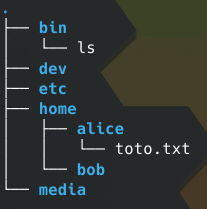
\includegraphics[scale=.6]{pics/pic_01.png}}}
                
                \vspace{6pt}
                
                $-$ \texttt{bin} : éxécutables permettant de démarrer le système et commandes de terminal ;
                
                $-$ \texttt{dev} : interfaces vers des périphériques ;
                
                $-$ \texttt{etc} : les fichiers de configuration du système ;
                
                $-$ \texttt{home} : répertoires personnels des utilisateurs ;
                
                $-$ \texttt{media} : les données des périphériques de stockage que l'on doit ``monter'' (brancher).
                
                \vspace{12pt}
                
                Chaque élément de l'arborescence est décrit par un chemin indiquant comment naviguer dans l'arborescence pour accéder au ficher.
                
                \vspace{12pt}
                
                \begin{indt}{Un chemin peut être}
                    $-$ \emph{Absolu} : c'est la suite des répertoires à traverser depuis la racine.
                    
                    Ex : \texttt{/home/alice/toto.txt}
                    
                    \vspace{6pt}
                    
                    $-$ \emph{Relatif} : c'est la suite des répertoires à traverser depuis le répertoire courant.
                    
                    Ex : depuis \texttt{home}, \texttt{alice/toto.txt}
                    
                    Depuis \texttt{bin} : \texttt{../home/alice/toto.txt}
                \end{indt}
                
                \vspace{12pt}
                
                \begin{indt}{Symboles :}
                    \texttt{.} désigne le répertoire courant ;
                    
                    \texttt{..} désigne le répertoire parent ;
                    
                    \texttt{$\sim$} désigne le répertoire personnel de l'utilisateur (répertoire courant par défaut)
                \end{indt}
            \end{indt}
            
            \vspace{6pt}
            
            \begin{indt}{\subsubsection{Manipulation de ficher depuis un programme}}
                Chaque langage a sa propre syntaxe pour les lectures et écritures dans des fichiers.
                
                \vspace{12pt}
                
                $\bullet$ En OCaml, il faut ouvrir un canal de communication / un flux de données avant de pouvoir lire ou écrire dans le ficher. Il faut penser à refermer ce canal.
                
                \begin{indt}{$-$ Type :}
                    \texttt{in\_channel} pour la lecture ;
                    
                    \texttt{out\_channel} pour l'écriture.
                \end{indt}
                
                \vspace{6pt}
                
                \begin{indt}{$-$ Ouverture d'un canal : on utilise les fonctions :}
                    \texttt{open\_in : string -> in\_channel} ;
                    
                    \texttt{open\_out : string -> out\_channel}
                
                    La chaîne de caractères en argument est un chemin (relatif / absolu) vers le ficher.
                \end{indt}
                
                \vspace{6pt}
                
                \begin{indt}{$-$ Fermeture d'un canal : on utilise les fonctions :}
                    \texttt{close\_in : in\_channel -> unit} ;
                    
                    \texttt{close\_out : out\_channel -> unit}
                \end{indt}
                
                \vspace{6pt}
                
                \begin{indt}{$-$ \'Ecriture / lecture :}
                    On écrit dans un ficher grâce à la fonction
                    
                    \texttt{output\_string : out\_channel -> string -> unit}
                    
                    Ex :
                    \begin{lstlisting}[language=Caml, xleftmargin=100pt]
let oc = open_out "/home/alice/toto.txt" in
    output_string oc "bonjour\n";
    close_out oc\end{lstlisting}
                    
                    \vspace{6pt}
                    
                    On lit \textit{via} la fonction \texttt{input\_line : in\_channel -> string} qui lit une ligne du fichier et la renvoie sans le caractère de retour à la ligne.
                    S'il n'y a plus de ligne à lire, la fonction soulève l'exception \texttt{End\_of\_file}.
                    
                    Ex :
                    \begin{lstlisting}[language=Caml, xleftmargin=100pt]
let ic = open_in "/home/alice/toto.txt" in
try
    while true do
        let s = input_line ic in
        Printf.printf "%s\n" s
    done
with
| End_of_file -> close_in ic\end{lstlisting}
                \end{indt}
                \vspace{12pt}
                
                $\bullet$ En C : les flux de données sont manipulés \textit{via} des pointeurs.
                
                \begin{indt}{$-$ Ouverture :}
                    On utilise la fonction \texttt{fopen}, de prototype 
                    
                    \texttt{FILE* fopen(char path[], char mode[])}
                    
                    où \texttt{path} désigne un chemin vers le fichier et \texttt{mode} est le mode d'ouverture : \texttt{"r"} pour la lecture ou \texttt{"w"} pour l'écriture (autres modes H.P).
                    
                    Il faut vérifier que le résultat n'est pas \texttt{NULL}.
                \end{indt}
                
                \vspace{6pt}
                
                \begin{indt}{$-$ Fermeture :}
                    on utilise la fonction \texttt{fclose}, de prototype
                    
                    \texttt{void fclose(FILE* file)}
                \end{indt}
                
                \vspace{6pt}
                
                \begin{indt}{$-$ \'Ecriture / lecture :}
                    Pour l'écriture, in utilise la fonction \texttt{fprintf}, équivalente à \texttt{printf} avec un argument supplémentaire de type \texttt{FILE*} (en première position).
                
                    Ex :
                    
                    \begin{lstlisting}[language=Caml, xleftmargin=100pt]
fprintf(file, "%p\n", file);
fprintf(file, "%d\n", x + y);\end{lstlisting}
                
                    \vspace{6pt}
                    
                    On lit grâce à la fonction \texttt{fscanf}, qui fonctionne comme \texttt{scanf} avec un argument supplémentaire que \texttt{fprintf}.
                    
                    On peut tester la valeur de retour de \texttt{fscanf} pour savoir si on a atteint la fin du fichier (valeur spéciale \texttt{EOF})
                    
                    Ex :
                    
                    \begin{lstlisting}[language=C, xleftmargin=100pt]
FILE* file = fopen("toto.txt", "r");
if (file == NULL) {
    printf("open failed\n");
    assert false;
}

char s[81];

while (fscanf(file, "%s", s) != EOF)
    printf("%s\n", s);
fclose(file);\end{lstlisting}
                    \vspace{6pt}
                    
                    \begin{indt}{Rq : \texttt{printf} et \texttt{scanf} sont les équivalents de \texttt{fprintf} et \texttt{fscanf} où l'on utilise le flux standard :}
                        $-$ \texttt{stdin} : flux d'entrée standard ;
                        
                        $-$ \texttt{stdout} : flux de sortie standard ;
                        
                        $-$ \texttt{stderr} : flux d'erreur standard, souvent égal à \texttt{stdout}.
                    \end{indt}
                    
                    \vspace{6pt}
                    
                    OCaml dispose aussi des flux standards, de mêmes noms. Il y a aussi une fonction \texttt{Printf.printf} en OCaml.
                \end{indt}
            \end{indt}
            
            \vspace{6pt}
            
            \begin{indt}{\subsubsection{Implémentation de l'arborescence de fichiers}}
                \begin{indt}{Dans les exemples précédants, on a accédé au contenu des fichiers de manière séquentielle. En pratique, la mémoire est organisée en blocs auxquels on peut accéder :}
                    $-$ directement, \textit{via} leur adresse en mémoire ;
                    
                    $-$ séquentiellement : on parcourt les blocs successifs à partir d'un bloc départ.
                \end{indt}
                
                \vspace{6pt}
                
                Les accès séquentiels sont en général plus rapides que les accès directs. Dans l'idéal, les fichiers seraient donc stockés dans des blocs contigus. Seulement, il y a un problème de fragmentation de la mémoire : les modifications successives de l'arborescence (création / suppression / redimmentionnement des fichiers) laissent des plages de blocs innutilisables. De plus, la gestion des blocs dépend du système de fichiers utilisé : le système d'exploitation n'applique pas la même stratégie pour éviter la fragmentation selon le système de fichier.
                
                Nous allons voir le principe de l'allocation indexée, utilisée dans les systèmes type UNIX.
                
                Un fichier est en fait un nom associé à un noeud d'index (inode) qui est une structure codée dans un / plusieurs blocs de mémoire et contenant les métadonnées du fichier (\textit{cf} 2.1.4) et les adresses des différents blocs contenant les données du fichier.
                
                Cela résout le problème de fragmentation (tout bloc devient utilisable en mettant à jour le noeud d'index du fichier concerné) sans trop réduire les performances des accès aux fichiers.
                
                Un répertoire est alors une liste de noeuds d'index associés à des noms. La séparation du nom des autres métadonnées est importante pour partager les blocs de mémoire associés à un fichier entre plusieurs noms, vus comme des ``raccourcis''.
                
                \begin{indt}{Il y a deux manières de procéder :}
                    $-$ Le lien physique (hard link) : on crée deux noms pour le \textit{même} noeud d'index.
                    
                    Il y a des restrictions : pas de lien physique vers des répertoires, ni vers un autre système de fichier.
                    
                    \vspace{6pt}
                    
                    $-$ Le lien symbolique (symbolic link) :  un lien symbolique est un nouveau fichier, donc un noeud d'index différent, ne contenant dans ses données que le chemin vers le fichier auquel il fait référence. Les restrictions des liens physiques ne s'appliquent pas aux liens symboliques.
                \end{indt}
            \end{indt}
            
            \vspace{6pt}
            
            \begin{indt}{\subsubsection{Attributs des fichiers}}
                Les attributs ou métadonnées, qui sont stockés dans le noeud d'index d'un fichier fournissent des informations sur le fichier.
                
                \begin{indt}{Dans la norme POSIX, on y trouve en particulier :}
                    $-$ La taille du fichier (en octets) ;
                    
                    $-$ Le nombre de blocs alloués ;
                    
                    $-$ Le nombre de liens physiques vers le noeud d'index ;
                    
                    $-$ Le numéro de l'index ;
                    
                    $-$ Les identifiants de l'utilisateur propriétaires et du groupe du fichier ;
                    
                    $-$ Des données d'horodatage concernant les accès et modifications du fichier ;
                    
                    $-$ Les droits d'accès au fichier, identifiant les opérations autorisées sur ce fichier selon l'utilisateur.
                \end{indt}
                
                \vspace{6pt}
                
                \begin{indt}{Il y a trois catégories d'utilisateur :}
                    $-$ Le proriétaire du fichier ;
                    
                    $-$ Les membres du groupe du fichier ;
                    
                    $-$ Les autres.
                \end{indt}
                
                \vspace{6pt}
                
                \begin{indt}{Pour chaque catégorie, il est possible d'autoriser ou d'interdire 3 opérations :}
                    $-$ La \emph{lecture} du fichier ;
                    
                    $-$ L'\emph{écriture} du fichier ;
                    
                    $-$ L'\emph{exécution} du fichier en tant que programme exécutable.
                \end{indt}
                
                \vspace{6pt}
                
                \begin{indt}{Cas particulier pour les répertoires :}
                    $-$ L'accès en lecture permet de lister le contenu du répertoire ;
                    
                    $-$ L'accès en écriture permet de créer / supprimer / renommer les fichiers contenus dans le répertoire (nécessite l'accès en exécution) ;
                    
                    $-$ L'accès en exécution permet de traverser le répertoire, i.e d'accéder au contenu du répertoire pour les fichiers pour lesquels on a des droits d'accès.
                \end{indt}
            \end{indt}
        \end{indt}
        
        \vspace{12pt}
        
        \begin{indt}{\subsection{Manipulations depuis le terminal}}
            \begin{indt}{\subsubsection{Navigation dans l'arborescence de fichiers}}
                $\bullet$ Se repérer : l'environement du terminal est placé dans un répertoire \textit{courant}. On utilise la commande \texttt{\em pwd} (\textit{print working directory}) pour déterminer le répertoire courant.
                
                Pour connaître le contenu d'un répertoire, on utilise la commande \texttt{\em ls} (\textit{list}).
                
                \begin{indt}{Deux options}
                    $-$ Sans argument, la commande liste le contenu du répertoire courant ;
                    
                    $-$ On peut passer en argument un chemin relatif / absolu vers un répertoire et la commande liste alors le contenu de ce répertoire.
                \end{indt}
                
                Ex :
                \begin{lstlisting}[language=Bash, xleftmargin=80pt]
ls /home/Alice
ls Bureau #Or Desktop
ls ../tp\end{lstlisting}
                
                \vspace{12pt}
                
                $\bullet$ Se déplacer : on utilise la commande \texttt{\em cd} (\textit{change directory}) pour changer de répertoire courant.
                
                Sans argument, cette commande déplace le répertoire courant vers le répertoire utilisateur (\texttt{$\sim$} : \texttt{/home/user}).
                
                On peut choisir le répertoire courant en donnant un chemin vers un répertoire.
                
                Ex :
                \begin{lstlisting}[language=Bash, xleftmargin=80pt]
cd ../..
cd ~
cd Bureau
cd ~/git/coursCPGE\end{lstlisting}


            \end{indt}
            
            %\vspace{6pt}
            \newpage
            
            \begin{indt}{\subsubsection{Modifications de l'arborescence de fichiers}}
                \begin{indt}{$\bullet$ Création de fichiers}
                    $-$ Fichiers : On peut utiliser un éditeur de texte (ex : commande \texttt{vim}, ou \texttt{emacs}).
                    
                    On peut également créer un fichier vide à l'aide de la commande \texttt{\em touch}, qui prend en argument un chemin vers le fichier à créer.
                    
                    Ex :
                    \begin{lstlisting}[language=Bash, xleftmargin=100pt]
touch DS/ds_03.tex
touch toto.txt\end{lstlisting}
                    
                    Si le fichier existe déjà, la commande modifie les métadonnées d'horodatage.
                    
                    \vspace{12pt}
                    
                    $-$ Répertoire : on crée un répertoire à l'aide de la commande \texttt{\em mkdir} (\textit{make directory}).
                    
                    Ex :
                    \begin{lstlisting}[language=Bash, xleftmargin=100pt]
mkdir /tmp/test\end{lstlisting}
                    
                    \vspace{12pt}
                    
                    $-$ Copie : on peut copier un fichier ou un répertoire à l'aide de la commande \texttt{\em cp} (\textit{copy}) qui prend en arguments un chemin vers le fichier / répertoire source et un chemin vers la destination.
                    
                    Ex :
                    \begin{lstlisting}[language=Bash, xleftmargin=100pt]
cp toto.txt ~/Bureau
cp toto.txt ~/Bureau/bla.txt
cp bla.txt bli.txt\end{lstlisting}
                    
                    Pour les répertoires, on doit utilier l'option \texttt{-r} (\textit{recursive}).
                    
                    Ex :
                    \begin{lstlisting}[language=Bash, xleftmargin=100pt]
cp -r /tmp ~/Documents
cp -r /tmp ~/Documents/copie_tmp #If copie_tmp don't exists, copy create copie_tmp in ~/Documents and /tmp/* in copie_tmp\end{lstlisting}
                \end{indt}
                
                \vspace{12pt}
                
                \begin{indt}{$\bullet$ Suppression :}
                    $-$ Fichiers : on supprime un fichier grâce à la commande \texttt{\em rm} (\textit{remove}) qui prend en argument un chemin vers le fichier à supprimer.
                    
                    Ex :
                    \begin{lstlisting}[language=Bash, xleftmargin=100pt]
rm /tmp/toto.txt\end{lstlisting}
                    
                    On peut donner plusieurs chemins pour supprimer plusieurs fichiers, et on dispose du symbole \texttt{*}, qui représente n'importe quelle chaîne de caractères.
                    \begin{lstlisting}[language=Bash, xleftmargin=100pt]
rm *.ml #Delete all files in current working directory with the .ml extension.
rm tp_*.c\end{lstlisting}
                    
                    \vspace{12pt}
                    
                    $-$ Répertoires : on supprime un répertoire \textit{vide} à l'aide de la commande \texttt{rmdir} (\textit{remove directory}). Plutôt que de vider un répertoire pour utiliser \texttt{rmdir}, on utilise plutôt l'option \texttt{-r} de \texttt{rm} : \texttt{\em rm -r [DIR...]}.
                    
                    Rq : on peut aussi utiliser \texttt{rm -d [empty\_dir...]} pour supprimer un répertoire vide.
                \end{indt}
                
                \vspace{12pt}
                
                \begin{indt}{$\bullet$ Déplacement :}
                    On déplace un fichier à l'aide de la commande \texttt{\em mv} (\textit{move}) prenant les mêmes arguments que \texttt{cp}.
                    
                    Pas d'option \texttt{-r}.
                \end{indt}
            \end{indt}
            
            \vspace{12pt}
            
            \begin{indt}{\subsubsection{Gestion des systèmes de fichier}}
                $\bullet$ Ajout d'un système de fichier : on utilise la commande \texttt{mount} (on parle de montage), qui prend en arguments un chemin vers le périphérique, et un chemin vers le répertoire qui contiendra l'arborescence du prériphérique.
                Sans arguments, la commande \texttt{mount} liste les points de montage.
                
                Ex :
                \begin{lstlisting}[language=Bash, xleftmargin=80pt]
mount /dev/sdc1 Document/my_USB_key\end{lstlisting}
                
                \vspace{12pt}
                
                $\bullet$ Démontage : on utilise la commande \texttt{umount}, qui prend en argument un chemin vers le point de montage.
            \end{indt}
            
            \vspace{12pt}
            
            \begin{indt}{\subsubsection{Gestion des droits}}
                $\bullet$ Exécuter une commande en tant qu'administrateur : on préfixe la commande par la commande \texttt{\em sudo} (\textit{super user do}).
                
                Ex :
                \begin{lstlisting}[language=Bash, xleftmargin=80pt]
sudo apt upgrade\end{lstlisting}
                
                L'utilisateur doit faire partie du groupe sudo, \textit{aka} les \textit{sudoers}.
                
                \vspace{12pt}
                
                $\bullet$ Gérer les droits des fichiers / répertoires : on représente les droits d'accès par une chaîne de caractères \texttt{rwxrwxrwx}, en plaçant des \texttt{-} pour les droits non attribués. Les trois premiers caractères représentent les droits de l'utilisateur, les trois suivants le groupe, et les trois derniers les autres.
                
                Ex : \texttt{rwxrw-r--}
                
                \begin{indt}{On peut changer cette chaîne à l'aide de la commande \texttt{\em chmod} (\textit{change mode}) qui peut être utilisée de 2 manières :}
                    $-$ On modifie les droits d'une catégorie (\texttt u pour utilisateur, \texttt g pour groupe, \texttt o pour les autres) par ajout (\texttt +), suppression (\texttt -) ou définition (\texttt =) de droits.
                    
                    Ex :
                    \begin{lstlisting}[language=Bash, xleftmargin=100pt]
chmod u+rw <path>
chmod o=r <path>\end{lstlisting}
                    
                    \vspace{12pt}
                    
                    $-$ On utilise une représenation numérique des droits (4 pour la lecture, 2 pour l'écriture, et 1 pour l'exécution) que l'on somme pour chaque catégorie.
                    
                    Ex :
                    \begin{lstlisting}[language=Bash, xleftmargin=100pt]
chmod 751 <path> # 7 for u : 4+2+1 ; 5 for g : 4+1 ; 1 for o.\end{lstlisting}
                \end{indt}
            \end{indt}
            
            \vspace{12pt}
            
            \begin{indt}{\subsubsection{Création de liens}}
                On utilise la commande \texttt{\em ln} (\textit{link}) qui prend les mêmes arguments que \texttt{cp} et \texttt{mv}.
                Par défaut, le lien est physique. Pour obtenir un lien symbolique, on utilise l'option \texttt{-s}.
                
                Ex :
                \begin{lstlisting}[language=Bash, xleftmargin=80pt]
ln -s /dev/sdb ~/Documents/data
ln tp/macros.tex td/\end{lstlisting}
            \end{indt}
            
            \vspace{12pt}
            
            \begin{indt}{\subsubsection{Redirection}}
                On peut rediriger les flux d'entrée / sortie des programmes.
                
                $\bullet$ Rediriger la sortie vers un fichier : on utilise \texttt > pour la sortie standard et \texttt{2>} pour la sortie d'erreur.
                
                Ex :
                \begin{lstlisting}[language=Bash, xleftmargin=80pt]
./prog 2> erreur.log
echo bonjour > /tmp/bonjour.txt\end{lstlisting}
                
                On utilise \texttt{>>} et \texttt{2>>} pour ajouter à la fin sans écraser le contenu.
                
                \vspace{12pt}
                
                $\bullet$ Rediriger l'entrée vers un fichier : on utilise \texttt <
                
                Ex :
                \begin{lstlisting}[language=Bash, xleftmargin=80pt]
ls > contenu.txt
sort < contenu.txt > sorted_content.txt\end{lstlisting}
                
                \vspace{12pt}
                
                $\bullet$ Rediriger la sortie d'un programme vers l'entrée d'un autre : on utilise un \textit{pipe} (tube en français), dénoté par \texttt{|}.
                
                Ex :
                \begin{lstlisting}[language=Bash, xleftmargin=80pt]
ls | sort > sorted_content.txt
ls | grep ".ml$"\end{lstlisting}
                
                %a
            \end{indt}
        \end{indt}
        
    \end{indt}
    
    \vspace{12pt}
    
    \begin{indt}{\section{Représentation de l'information : types numériques}}
        
        \begin{indt}{\subsection{Représentation des entiers}}
            \begin{indt}{\subsubsection{Intro}}
                En machine, les données sont stockées sous forme binaire, \textit{i.e} sous la forme de suites de 0 et de 1. Cela fonctionne car de nombreux types d'information peuvent être encodés par des entiers, qui eux-mêmes ont plusieurs représentations, dont la représentation binaire.
            \end{indt}
            
            \vspace{-12pt}
            
            \begin{indt}{\subsubsection{Bases de numération}}
                \begin{indt}{\textbf{Théorème :}}
                    Soit $b \in \N\ \backslash\ \{0\ ;\ 1\}$.
                    
                    Alors
                    
                    $
                        \forall n \in \N,\ \exists!\ (n_k)_{k \in \N}
                        \quad \text{tq}\ 
                        \begin{cases}
                            \forall k \in \N,\ n_k \in \nset{0}{b-1}
                            \\
                            (n_k)_{k \in \N}\ \text{stationne ultimement en } 0
                            \\
                            \displaystyle n = \sum_{k \in \N} n_k b^k = \sum_{k = 0}^p n_k b^k \quad \text{avec $p$ tq } \forall k > p,\ n_k = 0
                        \end{cases}
                    $
                    
                    \vspace{12pt}
                    
                    On appelle représentation en base $b$ la suite (finie) $n_p, \ldots, n_0$ et on note $n = \lrangle{n_p,\ \ldots, n_0}_b$
                \end{indt}
                    
                \vspace{12pt}
                
                $\square$
                
                \begin{indt}{$\bullet$ Unicité :}
                    On suppose l'existence d'un tel développement.
                    
                    \[ n = \sum_{k = 0}^p n_k b^k \]
                    
                    On remarque que $\displaystyle n = \lr{\sum_{k = 1}^p n_k b^{k - 1}}b + n_0$, avec $0 \le n_0 < b$.
                    
                    Donc $n_0$ est nécessairement le reste de la division euclidienne de $n$ par $b$.
                    
                    On note $\displaystyle N_1 = \sum_{k = 1}^p n_k b^{k - 1}$ le quotient (aussi uniquement déterminé) et on recommence.
                    
                    On montre par récurrence que les $n_k$ sont uniquement déterminés.
                \end{indt}
                
                \vspace{12pt}
                
                \begin{indt}{$\bullet$ Existence}
                    Si $n = 0$ : $(0)_{k \in \N}$ convient.
                    
                    Si $n > 0$ : on définit les suites $(n_k)_{k \in \N}$ et $(N_k)_{k \in \N}$ par
                    
                    $N_0 = n$
                    
                    $
                        \forall k \in \N,\ 
                        \begin{cases}
                            n_k\ \text{est le reste dans la division euclidienne de $N_k$ par $b$}
                            \\
                            N_{k + 1}\ \text{est le quotient dans la division euclidienne de $N_k$ par $b$}
                        \end{cases}
                    $
                    
                    \vspace{6pt}
                    
                    Par définition, $\forall k \in \N, \ n_k \in \nset{0}{b - 1}$.
                    
                    \vspace{-24pt}
                    
                    \begin{eqnarray*}
                        n &=& N_0
                        \\
                        &=& N_1 \cdot b + n_0
                        \\
                        &=& (N_2 \cdot b + n_1) + n_0 = N_2 \cdot b^2 + n_1 \cdot b + n_0
                    \end{eqnarray*}
                    
                    Une récurrence (finie) permettra de démontrer $\displaystyle n = \sum_{k \in \N} n_k b^k$ quand on aura montré que $(n_k)_{k \in \N}$ stationne en 0 à partir d'un certain rang.
                    
                    \vspace{12pt}
                    
                    Soit $k \in \N$.
                    
                    $N_k = b N_{k + 1} + n_k$ et $b > 1$
                    
                    Donc $2 N_{k + 1} \le b N_{k + 1} \le N_k$
                    
                    Donc par récurrence, $2^k N_k \le N_0 = n$
                    
                    Donc, pour $k$ tq $2^k > n$, $N_k = 0$ et $\forall p \ge k + 1,\ n_p = 0$
                \end{indt}
                
                $\blacksquare$
                
                \vspace{12pt}
                
                Ex :
                
                $b = 10$ : représentation binaire ;
                
                $b = 2$ : représentation binaire ;
                
                $b = 16$ : représentation hexadécimale : on utilise comme ``chiffres'' les symboles
                
                \texttt{0123456789abcdef}.
                
                \vspace{12pt}
                
                \begin{tabular}{|c|c|c|}
                    \hline
                    décimal & binaire & hexadécimal
                    \\
                    \hline
                    17 & 10001 & 11
                    \\
                    \hline
                    15 & 1111 & f
                    \\
                    \hline
                    0 & 0 & 0
                    \\
                    \hline
                \end{tabular}
            \end{indt}
            
            \vspace{12pt}
            
            \begin{indt}{\subsubsection{Remarques}}
                $-$ Il y a aussi une représentation unaire (base 1).
                
                \vspace{6pt}
                
                $-$ Les aglorithmes vu en primaire s'adaptent à toutes les bases.
                
                \vspace{6pt}
                
                $-$ Mais en pratique, on ne peut pas représenter tous les entiers : il y a un nombre maximal de chiffres. Si le résultat d'une opération doit utiliser plus de chiffres, il est tronqué (ce qui revient à faire des calculs modulos $b^p$ où $p$ est la taille maximale). On appelle cela un dépassement de capacité (\textit{overflow} en anglais).
                
                \vspace{6pt}
                
                \begin{indt}{$-$ La gestion des entiers négatifs nécessite un choix de représentation. Types en C :}
                    $\bullet$ Taille fixée explicitement : \texttt{int8\_t}, \texttt{int32\_t}, \texttt{int64\_t} pour les entiers relatifs ;
                    
                    \texttt{uint8\_t}, \texttt{uint32\_t}, \texttt{uint64\_t} pour les entiers naturels.
                    
                    On parle d'entiers non signés (unsigned).
                    
                    \vspace{6pt}
                    
                    $\bullet$ Si la taille importe peu : \texttt{int} et \texttt{unsigned int} (dont la taille est généralement 32 bits).
                \end{indt}
            \end{indt}
            
            \vspace{12pt}
            
            \begin{indt}{\subsubsection{Entiers signés}}
                $-$ Solution naïve : on utilise un bit de signe (0 pour positif, 1 pour négatif).
                
                Pb : on a 2 représentations de 0 ;
                
                Les aglorithmes usuels ne fonctionnent plus :
                
                $4 + (-2) = 2$ mais $\underbrace{\lrangle{0000\ 0100}_2}_4 + \underbrace{\langle 1000\ 0010 \rangle_2}_{-2} = \underbrace{\langle 1000\ 0110 \rangle_2}_{-6} $
                
                \vspace{12pt}
                
                $-$ Complément à 2 : sur $p$ bits, les entiers entre $-2^{p - 1}$ et $2^{p - 1} - 1$, représentés de manière unique.
                
                Idée : on note $\hat n$ le complémentaire de $n$ (en inversant les bits)
                
                Alors $n + \hat n = \langle 1 \ldots 1 \rangle_2 = 2^p - 1$
                
                donc $\hat n + 1 = 2^p - n \equiv -n\ [2^p]$
                
                \vspace{6pt}
                
                Si $n \ge 0$, on le représente normalement ;
                
                Si $n < 0$, on le représente par $\hat n + 1$, \textit{i.e} $2^p - \abs n$
                
                Ex :
                $6 + (-6) = 0$
                
                et $\langle 0000\ 0110 \rangle_2 + \langle 1111\ 1010 \rangle_2 = \langle 1\ 0000\ 0000 \rangle_2 = \langle 0000\ 0000 \rangle_2$ par \textit{overflow}.
            \end{indt}
        \end{indt}
            
        %\vspace{12pt}
        
        \begin{indt}{\subsection{Représentation des réels}}
            \begin{indt}{\subsubsection{Idée}}
                On s'inspire des bases de numération par les entiers et on représente séparément les parties entière et décimale :
                
                $\displaystyle \langle x_p \ldots x_0\ .\ x_{-1} \ldots x_{-q} \rangle_b = \sum_{k = -q}^p x_k b^k$
                
                Ex : $\langle 4.35 \rangle_{10} = 4 \pt{0} + 3 \pt{-1} + 5 \pt{-2}$
                
                $\langle {10}.11 \rangle_2 = 2^1 + 2^{-1} + 2^{-2} = \langle 2.75 \rangle_{10}$
                
                Rq : une telle représentation n'est pas nécessairement finie.
                
                \vspace{6pt}
                
                On appelle nombre décimal (resp. dyadique) un nombre dont la représentation en base 10 (resp. 2) est finie.
                
                \vspace{6pt}
                
                Calcul de la représentation :
                
                Soit $x \in\ ]0\ ;\ 1[$. On veut écrire $x$ sous la forme $\langle 0.x_{-1} x_{-2} \ldots \rangle_b$.
                
                On remarque que $b \cdot x = \langle x_{-1}\ .\ x_{-2} x_{-3} \ldots \rangle_b$ donc $x_{-1} = \lfloor bx \rfloor$
                
                Comme $x_{-1} - \lfloor bx \rfloor = \langle 0\ .\ x_{-2} x_{-3} \ldots \rangle_b$, on peut recommencer.
                
                \vspace{6pt}
                
                Exemple :
                
                $\langle 0.7 \rangle_{10}$ en base 2 ?
                
                $2 \times 0.7 = 1.4 \rightarrow 1$
                
                $2 \times 0.4 = 0.8 \rightarrow 0$
                
                $2 \times 0.8 = 1.6 \rightarrow 1$
                
                $2 \times 0.6 = 1.2 \rightarrow 1$
                
                $2 \times 0.2 = 0.4 \rightarrow 0$
                
                $\langle 0.10110\ 0110\ 0110 \ldots \rangle_2$
                
                \vspace{12pt}
                
                Rq : pour utiliser cette représentation, on fixe les nombres de chiffres avant et après la virgule. On parle de représentation de virgule fixe.
            \end{indt}
            
            \vspace{12pt}
            
            \begin{indt}{\subsubsection{Représentation en virgule flottante}}
                On s'inspire de la représentation scientifique des nombres.
                
                \vspace{6pt}
                
                $x = (-1)^s \cdot m \cdot 2^e$ où :
                
                $s \in \{0\ ;\ 1\}$ est le bit de signe ;
                
                $m \in [1\ ;\ 2[$ est la mantisse ;
                
                $e \in \mathbb{Z}$ est l'exposant.
                
                \vspace{6pt}
                
                Rq : on ne peut pas représenter 0.
                
                La représentation binaire de $m$ est de la forme $\langle 1.m_{-1} m_{-2} \ldots \rangle_2$.
                
                On fait des erreurs d'arrondi si $m$ n'est pas dyadique.
                
                \vspace{12pt}
                
                Norme \texttt{IEEE-754} : établie en 1985, elle définit une convention sur la représentation des nombres en virgule flottante.
                
                \begin{tabular}{|r|c|c|c|c|p{100pt}|}
                    \hline
                    & Nb bits & Signe & Exposant & Mantisse & Type
                    \\
                    \hline
                    Simple précision
                    & 32
                    & 1
                    & 8
                    & 23
                    & \texttt{float} en C
                    \\
                    \hline
                    Double précision
                    & 64
                    & 1
                    & 11
                    & 52
                    & \texttt{double} en C, \texttt{float} en OCaml
                    \\
                    \hline
                \end{tabular}
                
                Convention : on ne stocke pas la partie entière de la mantisse
                
                l'exposant $e$ est représenté par l'écriture binaire de $e + 2^{p - 1} - 1$ où $p$ est le nombre de bits d'exposant.
                
                Attention, pas de complément à 2.
                
                Ex : en simple précision : \texttt{0 1000 0010 1100 0000 0000 0000 0000 000}
                
                $s = 0$ nombre positif
                
                $e = \langle 1000\ 0010 \rangle_2 - 2^7 + 1 = 130 - 127 = 3$
                
                $m = \langle 1.11 \rangle_2 = \langle 1.75 \rangle_{10}$
                
                Donc $x = +1.75 \cdot 2^3 = 14$
                
                \vspace{12pt}
                
                Rq : En raison des erreurs d'approximation, on ne teste jamais l'égalité de 2 flottants. On compare plutôt la valeur absolue de leur différence à l'erreur liée à leur précision.
                
                Ex : en simple précision l'erreur est de l'ordre de $2^e \cdot 2^{-23}$ donc on compare à $10^{-7}$
                
                En double précision, on compare à $10^{-16}$
                
                \vspace{12pt}
                
                \begin{indt}{Cas particuliers de la norme \texttt{IEEE-754} :}
                    $-$ Si les bits d'exposant ne sont pas $0\ldots 0$ ou $1 \ldots 1$, on parle de forme normalisée ;
                    
                    \vspace{6pt}
                    
                    \begin{indt}{$-$ Si les bits d'exposant sont $1\ldots 1$ :}
                        $+$ Si les bits de la mantisse sont $0 \ldots 0$ : cela encode $\pm \infty$ selon le signe ;
                        
                        $+$ Si au moins un bit de mantisse vaut 1, cela encode \texttt{NaN} (Not a Number) ;
                    \end{indt}
                    
                    \vspace{6pt}
                    
                    $-$ Si les bits d'exposant sont $0 \ldots 0$, on parle de forme dénormalisée.
                    
                    Le nombre représenté est alors, avec $p$ bits d'exposant et $q$ bits de mantisse :
                    \[ (-1)^s \cdot m \cdot 2^e \]
                    où $e = 2 - 2^{p - 1}$ et $m = \langle 0.m_{-1}\ldots m_{-q} \rangle_2$.
                \end{indt}
            \end{indt}
        \end{indt}
        
    \end{indt}


    

    
    
\end{document}
%--------------------------------------------End
